\documentclass[11pt,a4paper]{article}
\usepackage{acl2015}
\usepackage{times}
\usepackage{url}
\usepackage{latexsym}
\usepackage{tikz}
\usepackage{pgfplots}
\usepackage{pgfplotstable}
\usetikzlibrary{bayesnet}
\usepackage{caption}
\usepackage{subcaption}
\usepackage{graphicx}
\graphicspath{ {images/} }
\setlength\titlebox{5cm}

\title{Sentence Level Predictions With Path Ranking Algorithm}

\author{Dheeru Dua \\
  Carnegie Mellon University \\
  {\tt ddua@andrew.cmu.edu} \\\And
  Matt Gardner \\
  Carnegie Mellon University \\
  {\tt mg1@cs.cmu.edu} \\}

\date{}

\begin{document}
\maketitle
\begin{abstract}

The focus of Artificial Intelligence has always been to make machines
understand and comprehend text like humans do. This has induced active research
in the field of Information Extraction(IE) for better natural language
understanding. The availability of Knowledge bases like Freebase, Wikipedia has
facilitated this research on a large scale. Even though these KBs are large,
they have gaps in terms of coverage of facts.

In this paper, we try to bring forth the goodness of two techniques of relation
extraction in a coherent manner such that it beats the current state of the art
system. We augment Path Ranking Algorithm's~\cite{lao-2010-pra} power to
perform inference on incomplete KB with MultiR
algorithm's~\cite{hoffmann-2011-distant-supervision} abilities to extract
relations from sentence structure.

\end{abstract}

\section{Introduction}

Weak supervision is a promising approach when the availability of annotated
data is limited. We focus on a specific class of weakly supervised techniques
that uses Knowledge Bases like Freebase~\cite{freebase-2008-bollacker} to
heuristically extract knowledge from textual data. For instance, ``Pittsburgh
is located in Pennsylvania" is a ground truth which is represented in Freebase
as a tuple locatedIn(Pittsburgh, Pennsylvania).

\cite{riedel-2010-distant-supervision} proposed an ``atleast once" model which
learnt single relation from multiple sentence mentions of two entities.
However, \cite{riedel-2010-distant-supervision} assumes that two entities can
only be associated with each other by one relation. This leads to poor
performance of the relation extractors, in cases like locatedIn(Pittsburgh,
Pennsylvania) and secondLargestCityIn(Pittsburgh, Pennsylvania).
\cite{hoffmann-2011-distant-supervision} proposed MultiR algorithm to overcome
this problem.  Another problem with databases like Freebase is their
incompleteness and inaccuracy at times.

The Path Ranking Algorithm~\cite{lao-2010-pra} employs a combination of
constrained, weighted, random walks through the knowledge base graph to infer
new beliefs from the knowledge base.

We propose an approach that extends the feature space
of~\cite{riedel-2010-distant-supervision} with new beliefs learnt from Path
Ranking Algorithm to learn a perceptron-like online model with MultiR
algorithm.

Our model achieved huge improvements at both aggregate as well as sentence
level predictions when compared to the current state of the art techniques for
relation extraction.

\section{Multi-Instance learning with MultiR}

MultiR algorithm~\cite{hoffmann-2011-distant-supervision} is a probabilistic
graphical model for Multi-instance learning with distant supervision. We use
the dataset developed by~\cite{riedel-2010-distant-supervision}, aligning
Freebase relations with New York Times corpus.  The dataset contains a number
of sentence mentions for each entity pair. The entities are extracted from
sentences by Stanford Named Entity Tagger~\cite{finkel-2005-non-local-ie},
spanning across 52 freebase relations. The sentence level features include the
part of speech tags, named entities and dependency tree paths. An on-line
perceptron style model is then trained on 67946 such entity relation pairs. The
network structure is described in Figure 3a, where $S$ is the set of sentences
between any two entities $e_1$, $e_2$ $\in$ E and $Z_i$'s are the latent
variables that range over all relation names and a distinct value None. The
model outputs a binary relation vector Y, with indicator bits for each
relation. If their is a mistake in predicting the relation vector, weights are
appropriately adjusted in the parameter vector for each sentence mention of an
entity pair. Figure 1, shows a bipartite graph representing overlapping
relations between two entities in various sentence mentions.

\begin{figure}
  \begin{tikzpicture}

    \node[latent]            (z1) {\tiny None} ; %
    \node[latent, right=2.2cm of z1]            (z2) {\tiny locatedIn} ; %
    \node[latent, right=2.2cm of z2]            (z3) {\tiny locatedIn} ; %
    \node[latent, above=1cm of z1]  (yCapitalOf)   {$\mathbf{0}$}; %
    \node[latent, above right=1.2cm and 2.5cm of z1] (yLocatedIn)   {$\mathbf{1}$}; %
    \node[latent, above right=1.2cm and 2.5cm of z2] (yBornIn)   {$\mathbf{0}$}; %
    \node[const, above=0.1cm of yCapitalOf] (tagyCapitalOf)  {\small yCapitalOf} ; 
    \node[const, above=0.1cm of yLocatedIn] (tagyLocatedIn)  {\small yLocatedIn} ; %
    \node[const, above=0.1cm of yBornIn] (tagyBornIn)  {\small yBornIn} ; %
    \node[const, below=0.1cm of z1] (sentyCapitalOf)  {\small Pittsburgh is also called the Steel City.} ;
    \node[const, below=0.1cm of z2] (sentyLocatedIn)  {\small Pittsburgh is the second largest state in Pennsylvania} ; %
    \node[const, below=0.1cm of z3] (sentyBornIn)  {\small Pittsburgh is in the western part of Pennsylvania} ;

    \factor[above=0.5cm of z1] {yCapitalOf-f} {} {yCapitalOf} {z1,z2,z3} ; %
    \factor[above=0.5cm of z2] {yLocatedIn-f} {} {yLocatedIn} {z1,z2,z3} ;
    \factor[above=0.5cm of z3] {yBornIn-f} {} {yBornIn} {z1,z2,z3} ;


  \end{tikzpicture}
  \caption{Network for a pair of entities Pittsburgh and Pennsylvania}
  \label{fig:M1}
\end{figure}

\section{The Path Ranking Algorithm}

The Path Ranking Algorithm~\cite{lao-2010-pra}  is a general technique for
performing link prediction in a graph, however it has mainly been used for
knowledge base
completion~\cite{lao-2011-pra2,gardner-2013-latent-pra,gardner-2014-vector-space-pra}.
To learn a prediction model for a particular edge type in a graph, PRA finds
sequences of edge types (or paths) that frequently connect nodes that are
instances of the edge type being predicted. PRA then uses those path types as
features in a logistic regression model to infer missing edges in the graph.
PRA predicts the probability of landing on a target entity, $e_2$ starting from
an entity $e_1$, following a path type $\pi$: p($e_2|e_1$,$\pi$).For instance,
in Figure 2, we can find P(``the Mon"$|$ ``Pittsburgh",``lies on") based on the
graph connectedness by performing random walks.

\begin{figure}
  \begin{tikzpicture}
    \node [block] (sc) {\small Steel City};
    \node [block, right=2.5cm of sc] (ag) {\small the Alleghney};
    \path (sc) edge [->] node [above=0.2] {\small overlooks} (ag) ;


    \node [block, below=1.5cm of sc] (pt) {\small Pittsburgh};
    \node [block, above right=0.1cm and 2.5cm of pt] (mn) {\small the Mon};
    \node [block, below right=0.1cm and 2.5cm of pt] (mng) {\small the Monongahela};
    \path (pt) edge [->] node [above=0.2] {\small lies on} (mn) ;
    \path (pt) edge [->] node [above=0.2] {\small sits on} (mng) ;

  \end{tikzpicture}
  \caption{Graphical representation for sentences ``Steel City overlooks the
    Alleghney", ``Pittsburgh lies on the Mon", ``Pittsburgh sits on the
    Monongahela".}
  \label{fig:M1}
\end{figure}

\section{Related Work}

The first attempt of RE using weak or distant supervision was done
by~\cite{craven-1999-biological-kbs} to match the Yeast Protein Database with
abstracts in PubMed using a Naïve-Bayes extractor.

\cite{weston-2013-connecting-language-and-kb} made an attempt to utilize KB for
more than just relation mappings. They learnt scoring functions that operate by
learning low-dimensional embeddings of entities and relationships from KB
triples. In vector space analogy, each entity can be represented as a point and
each relationship is modeled as an operation like rotation, translation etc.
The correctness of a triple(entity-relationship-entity) is evaluated by
checking the compatibility of the two entities under the specified relation.
Their model is state of the art till date.

\begin{figure}[t!]
  \begin{subfigure}[t]{2.0cm}
    \begin{tikzpicture}
       \node[latent]          (y)   {$Y$};
       \node[latent, below=2cm of y]            (zi) {$Z_i$} ;
       \factor[below=1.2cm of y] {y-f} {} {y} {zi} ;
       \factor[right=0.3cm of zi] {zi-f} {$f_{s}$} {zi} {} ;
        \plate {r} {
          (y)
        } {$R$} ; %
       \plate {s} {
          (zi)(zi-f)
        } {$S$} ; %
      \plate {ee} {
          (r)(s)
        } {$EXE$} ; %
    \end{tikzpicture}
    \caption{MultiR}
  \end{subfigure}
  ~
  \begin{subfigure}[t]{2.0cm}
    \begin{tikzpicture}
       \node[latent]          (y)   {$Y$};
       \node[latent, below=2cm of y]            (zi) {$Z_i$} ;
       \factor[below=1.2cm of y] {y-f} {} {y} {zi} ;
       \factor[right=0.3cm of zi] {zi-f} {$f_{s}$} {zi} {} ;
       \factor[right=of y-f] {zi-fpra} {$f_{pra}$} {y-f} {} ;
        \plate {r} {
          (y)
        } {$R$} ; %
       \plate {s} {
          (zi)(zi-f)
        } {$S$} ; %
      \plate {ee} {
          (r)(s)
        } {$EXE$} ; %
    \end{tikzpicture}
    \caption{Per Entity-pair}
  \end{subfigure}
  ~
  \begin{subfigure}[t]{2.0cm}
    \begin{tikzpicture}
       \node[latent]          (y)   {$Y$};
       \node[latent, below=2cm of y]            (zi) {$Z_i$} ;
       \factor[below=1.2cm of y] {y-f} {} {y} {zi} ;
       \factor[right=0.3cm of zi] {zi-f} {$f_{s}$} {zi} {} ;
       \factor[left=0.3cm of zi] {zi-fpra} {$f_{pra}$} {zi} {} ;
        \plate {r} {
          (y)
        } {$R$} ; %
       \plate {s} {
          (zi)(zi-f)(zi-fpra)
        } {$S$} ; %
      \plate {ee} {
          (r)(s)
        } {$EXE$} ; %
    \end{tikzpicture}
    \caption{Per Mention}
  \end{subfigure}
  \caption{Plate notation of the model}
\end{figure}

\section{Methodology}

We augmented the features learnt from Path Ranking Algorithm with Sentential
features developed by~\cite{riedel-2010-distant-supervision} in two ways: at
sentence-mention level(Per Mention) and at entity-pair level(Per Entity-pair).
The graphical notation of both the models in reference to the baseline(MultiR)
are described in Figure 3. $f_{pra}$ are the direct or indirect path features
between two entities in the entire graph. These features are extracted by
performing random walks on the Freebase graph~\cite{lao-2011-pra2}. $f_{s}$ are
the sentence level features like dependency paths used
in~\cite{riedel-2010-distant-supervision,hoffmann-2011-distant-supervision,surdeanu-2012-relation-extraction}.
Each entity pair contains a set of sentence mentions S and Y is the binary
relation vector depicting relations between any two entities.


\subsection{Per Entity-pair}

In this model, we add PRA features once for an entity pair and not with each
sentence mention. This approach performs better over using only PRA features
(Figure 4) as it incorporates entity connectedness in freebase graph along with
the syntactic patterns entailing how language specific constructs can define
relation between two entities for instance ``The Monongahela river flows
through Pittsburgh, Pennsylvania" tells us that Pittsburgh is locatedIn
Pennsylvania.

\subsection{Per Mention}

In this model, we add PRA features per sentence mention in contrast to previous
case where we added the features per entity pair. This model performs better
over Per Entity-pair for two reasons.  First, it trains a better representation
of the model by bringing the semantic and syntactic components of the language
together in each parameter update. Secondly, in case of Per Entity-pair the
weights in parameter vector suggest that, most of the weight distribution goes
to PRA features causing the model learn a poor representation of the baseline
features.

\begin{figure}
  \centering
  \begin{tikzpicture}
    \begin{axis}[xlabel=Recall, ylabel=Precision, no markers,width=\columnwidth]
      \addplot table [y=Precision, x=Recall]{data/pra_per_mention.tsv};
      \addlegendentry{PRA Per Mention}
      \addplot table [y=Precision, x=Recall]{data/pra_per_entity.tsv};
      \addlegendentry{PRA Per Entity}
      \addplot [mark=none, green] table [y=Precision, x=Recall]{data/pra_only.tsv};
      \addlegendentry{PRA Only}
    \end{axis}
  \end{tikzpicture}
  \caption{Comparison between methods we introduced}
\end{figure}

\section{Experiments}

To evaluate our approach we compare the result of the model learnt with Per
Mention approach to the baseline MutliR
model~\cite{hoffmann-2011-distant-supervision} and few other models:
MIML~\cite{surdeanu-2012-relation-extraction};
WESTON~\cite{weston-2013-connecting-language-and-kb}) that followed MultiR. We
first run the Path Ranking Algorithm on the entire freebase graph excluding any
direct and inverse edges describing relations present in the training and
testing set. Then, we add these features to dataset developed
by~\cite{riedel-2010-distant-supervision} and train a model directly with
source code used in~\cite{hoffmann-2011-distant-supervision}. We found that
because of an increase in feature space w.r.t the number of training instances
model parameters do not generalize well and the model learnt is noisy. We
resort to using regularization to counter this problem and perform a 5 fold
cross validation with 80\%-20\% split of the training data to choose the
parameter for L2 regularization. Then, we average the values from 5 different
runs and use it to learn the final model for evaluation.


\subsection{Aggregate Performance}

The precision and recall are evaluated by comparing the set of relations
extracted against the entire set of input entity-pair and relations pairs in
the test set. The results are shown in Figure 5. Our model is computationally
efficient and performs better in comparison to
MIML~\cite{surdeanu-2012-relation-extraction} which uses a more complex
graphical model. We could not reproduce the results for MIML and WESTON
directly so we used a
digitizer\footnote{http://arohatgi.info/WebPlotDigitizer/} to extract the
values directly from the figures presented in the papers.

\begin{figure}
  \centering
  \begin{tikzpicture}
    \begin{axis}[xlabel=Recall, ylabel=Precision, no markers,width=\columnwidth]
      \addplot table [y=Precision, x=Recall]{data/hoffmann.tsv};
      \addlegendentry{Hoffmann}
      \addplot table [y=Precision, x=Recall]{data/weston.tsv};
      \addlegendentry{Weston}
      \addplot table [y=Precision, x=Recall]{data/pra_per_mention.tsv};
      \addlegendentry{Ours}
    \end{axis}
  \end{tikzpicture}
  \caption{Comparison with prior work}
  \label{fig:re-prior-work}
\end{figure}

\subsection{Sentence-Level Performance}

The performance is evaluated on a sample set of 1000 sentences which were
manually labeled and used in~\cite{hoffmann-2011-distant-supervision}. We
noticed that when we used PRA features only in the training instances and not
in the testing instances, the model performs even better. This shows that PRA
features help learn better sentence-level extractors which are more generic in
nature. Moreover, incompleteness of the Knowledge base will not hamper the
overall performance of the algorithm at test time. Figure 5 shows the
sentence-level results with and without PRA features in the test set in
comparison to baseline~\cite{hoffmann-2011-distant-supervision}.

\begin{figure}
  \centering
  \begin{tikzpicture}
    \node (fig4)
        {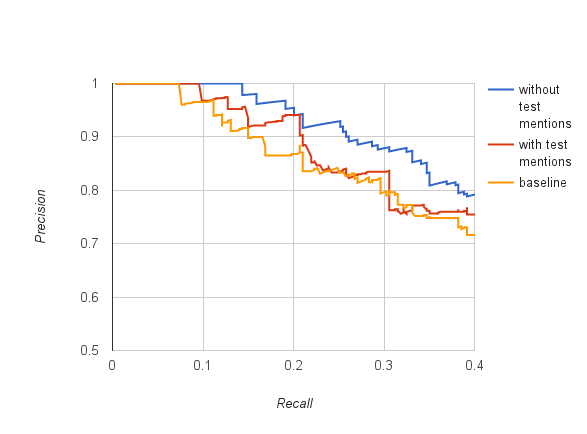
\includegraphics[width=8cm,height=7cm]{figure6.png}};
  \end{tikzpicture}
  \caption{Comparison between methods we introduced}
\end{figure}

\section{Discussion and Error Analysis}

Figure 6 shows how KB can help provide richer background information about the
entities referred to in text.  Moreover, our model introduces a very generic
way of injecting features into any graphical model representing pair-wise
factors between any two entities, ensuring no over-fitting.

Figure 4 and 5 indicate that our model outperforms existing state-of-the art
models at both sentence-level and aggregate-level performance.

On further analysing the sentence mentions which PRA helped in classifying
correctly from baseline, we found that PRA features provide a much stronger
evidences for prediction over dependency parse tree features when sentence
structures are very complex. For instance, for the text snippet taken from The
New York Times,

\begin{quote}
  Marlene Sehestedt or Rudy Stupar , United Country South Range Prime
  Properties (719) 948-2802 ; www.unitedcountry.com/puebloco Seattle WHAT :
  Two-bedroom condominium HOW MUCH : \$509,000 PER SQUARE FOOT : \$596.72 On
  the 21st floor of the 111-unit Grandview condominium , this 853-square-foot
  apartment in downtown Seattle has views of Lake Union , Mount Baker , Mount
  Rainier and the Space Needle ."
\end{quote}

PRA features help correctly predict that ``Mount Rainier'' is located in
``Seattle". The dependency-path features are unable to capture that information
for sentence-level prediction.

\begin{figure}
  \begin{tikzpicture}
    \node [block] (sc) {\small Steel City};
    \node [block, right=1.8cm of sc] (ag) {\small the Alleghney};
    \path (sc) edge [->] node [above=0.2] {\small overlooks} (ag) ;
    \node [block, right=1.8cm of ag] (agr) {\small Alleghney River};
    \path (ag) edge [->,red] node [above=0.2] {\small canReferTo} (agr) ;


    \node [block, below=1.5cm of sc] (pt) {\small Pittsburgh};
    \node [block, above right=0.1cm and 1.5cm of pt] (mn) {\small the Mon};
    \node [block, below right=0.1cm and 1.5cm of pt] (mng) {\small the Monongahela};
    \path (pt) edge [->] node [above=0.2] {\small lies on} (mn) ;
    \path (pt) edge [->] node [above=0.2] {\small sits on} (mng) ;
    \node [block, below right=0.1cm and 2.0cm of mn] (mngr) {\small Monongahela River};
    \path (mn) edge [->,red] node [above=0.2] {\small canReferTo} (mngr) ;
    \path (mng) edge [->,red] node [above=0.2] {\small canReferTo} (mngr) ;
    \path (sc) edge [->,red] node [right=0.1] {\small canReferTo} (pt) ;

  \end{tikzpicture}
  \caption{Graphical representation for sentences ``Steel City overlooks the
    Alleghney", ``Pittsburgh lies on the Mon", ``Pittsburgh sits on the
    Monongahela" augmented with Knowledge Base property ``canReferTo"}
  \label{fig:M1}
\end{figure}

\section{Conclusion}

In this paper we described a framework that leverages the Knowledge graph like
freebase to extract features from not just how the two entities of concern are
connected directly with each other, but also how they are connected via other
entities. This is generic way which can be used in knowledge base population
and entity linking tasks etc.

\bibliographystyle{acl}
\bibliography{bib}

\end{document}
